\section{Simulation Plan and Example Scenarios}

\subsection*{Simulation workflow}

\begin{enumerate}[label=\arabic*.]
    \item Implement the ODEs for $(L,E,M,P)$ and solve over $t\in[0,T]$ (e.g., 0--10 days) using a stiff-capable solver if $k_{\mathrm{loss},E}$ is large (common when modeling low escape).
    \item Compute interpretable summary metrics from $P(t)$:
    \begin{itemize}
        \item $P_{\max}$ (peak height)
        \item $t_{\mathrm{peak}}$ (time to peak)
        \item $\mathrm{AUC}_P$ (total antigen exposure)
        \item FWHM (full width at half maximum; duration near peak)
        \item time-above-threshold $T(P\ge P_{\mathrm{thr}})$ (immune-relevant persistence surrogate)
    \end{itemize}
    \item Perform scenario sweeps and local sensitivities on log-scaled parameters.
\end{enumerate}

\subsection*{Example baseline and scenario outcomes}

Using the baseline parameter set defined earlier (normalized dose), a simple numerical integration yields a single-peaked antigen curve with a peak near $\sim 1$ day and multi-day tail.

Below are model-generated metrics for several contrasting scenarios (all else held constant unless stated). These numbers are model outputs for illustration, not measured data.

\begin{table}[H]
    \centering
    \caption{Illustrative scenario comparison}
    \begin{tabular}{>{\raggedright\arraybackslash}p{0.48\textwidth}cccc}
        \toprule
        Scenario (change vs baseline) & Peak $P_{\max}$ & $t_{\mathrm{peak}}$ (h) & AUC$_P$ & FWHM (h) \\
        \midrule
        Baseline & 0.089 & 27.8 & 5.55 & 54.2 \\
        Fast mRNA decay $k_{\mathrm{deg}}=0.30$ & 0.034 & 19.7 & 1.85 & 45.5 \\
        Slow mRNA decay $k_{\mathrm{deg}}=0.03$ & 0.197 & 43.7 & 18.37 & 84.7 \\
        Low translation $k_{\mathrm{tl}}=0.3$ & 0.027 & 27.8 & 1.66 & 54.2 \\
        High translation $k_{\mathrm{tl}}=3.0$ & 0.267 & 27.8 & 16.64 & 54.2 \\
        Poor delivery (slow uptake) $k_{\mathrm{up}}=0.03$ & 0.051 & 38.0 & 3.99 & 70.0 \\
        Efficient delivery (fast uptake) $k_{\mathrm{up}}=0.30$ & 0.110 & 21.1 & 6.24 & 48.2 \\
        Lower escape $f_{\mathrm{esc}}=0.01$ & 0.044 & 27.7 & 2.77 & 54.2 \\
        Higher escape $f_{\mathrm{esc}}=0.10$ & 0.444 & 28.2 & 27.74 & 54.2 \\
        Fast protein clearance $k_{\mathrm{clr}}=0.10$ & 0.048 & 18.9 & 1.67 & 32.0 \\
        Slow protein clearance $k_{\mathrm{clr}}=0.01$ & 0.123 & 37.7 & 14.83 & 106.8 \\
        \bottomrule
    \end{tabular}
\end{table}

\begin{figure}[H]
    \centering
    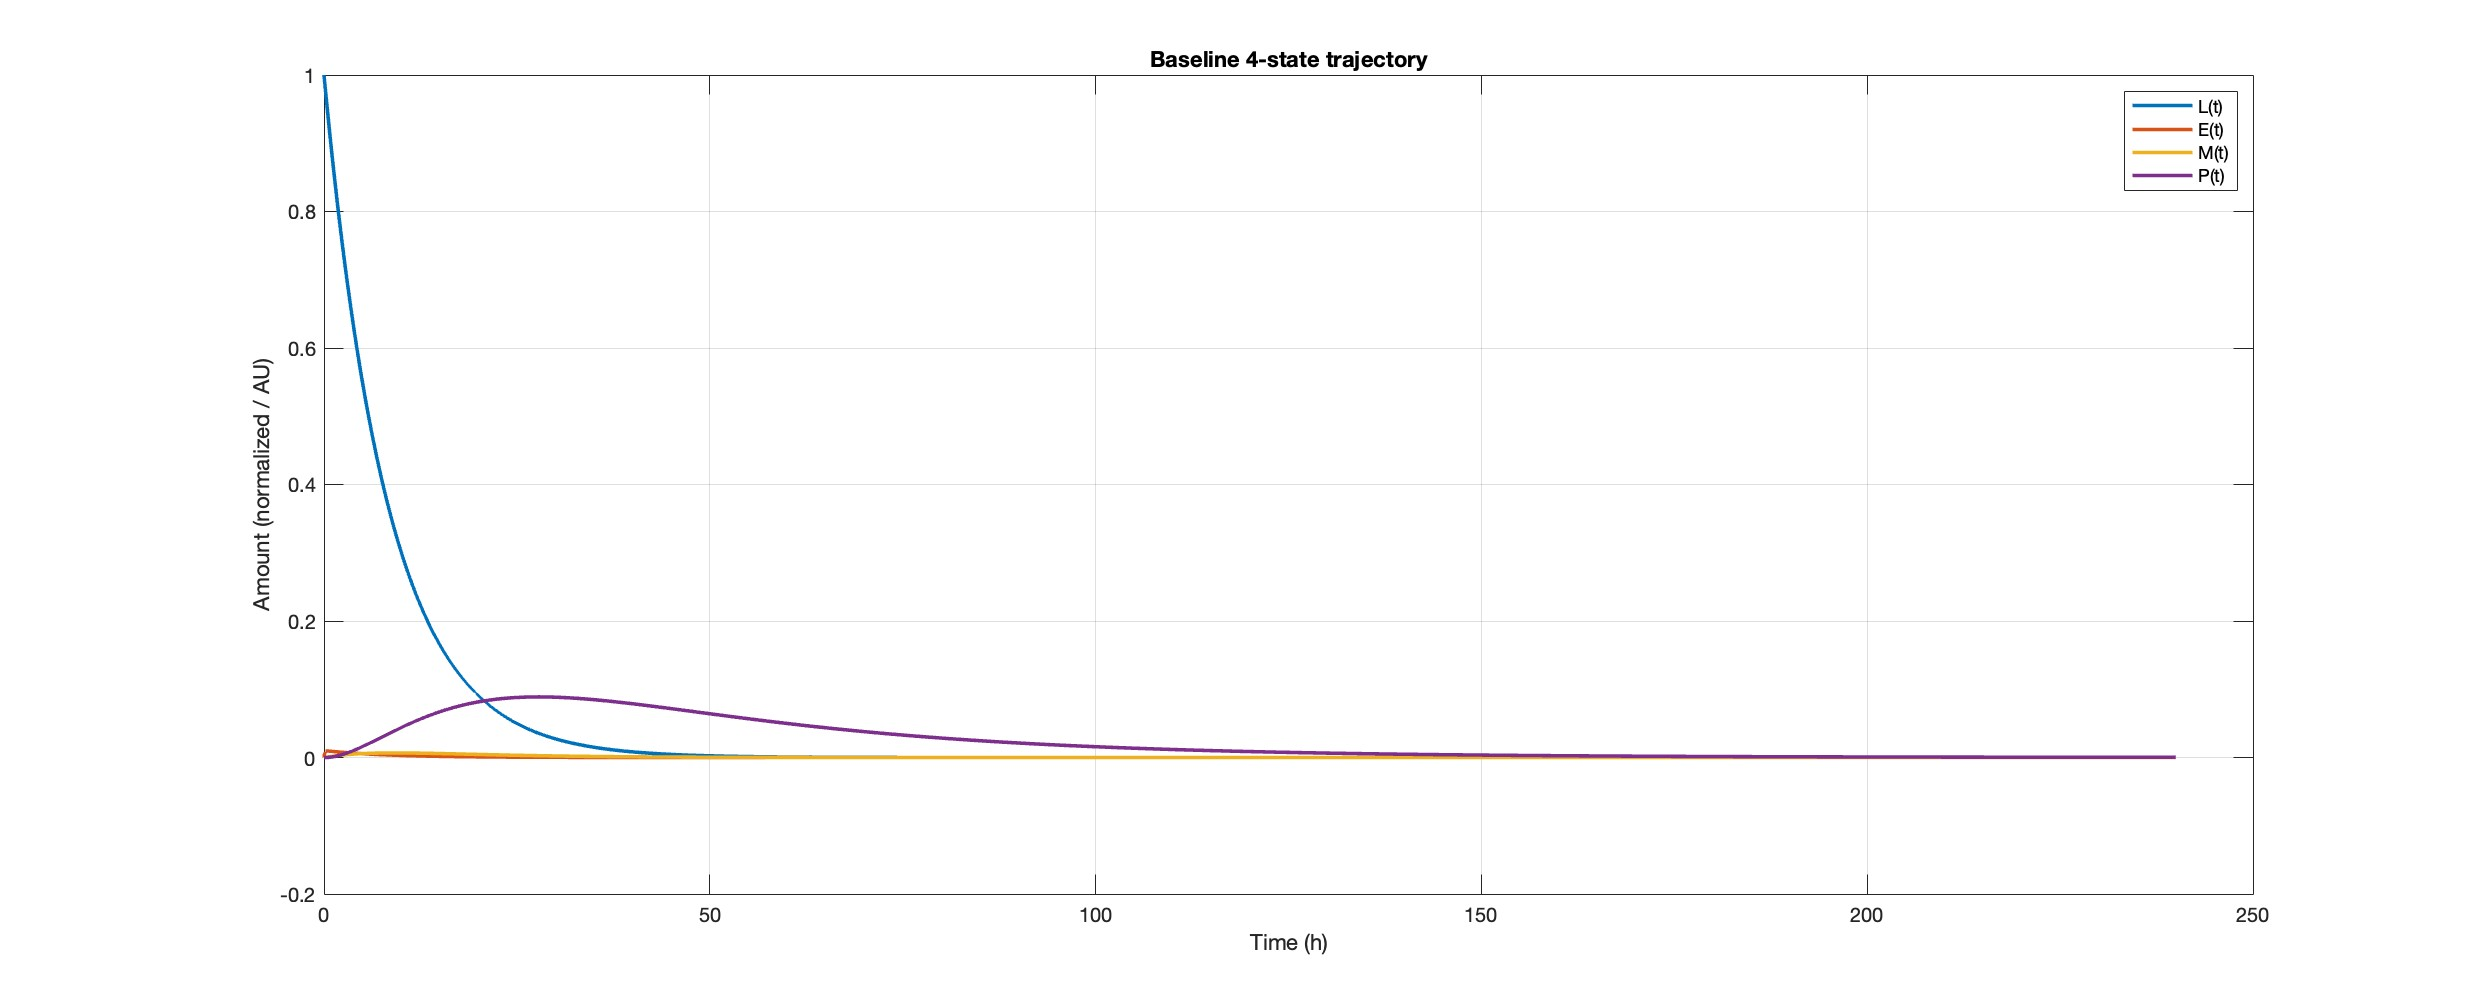
\includegraphics[width = \textwidth]{figures/Base_traj.jpg}
    \caption{Baesline 4-state trajectory}
    \label{fig:base_traj}
\end{figure}

\begin{figure}[H]
    \centering
    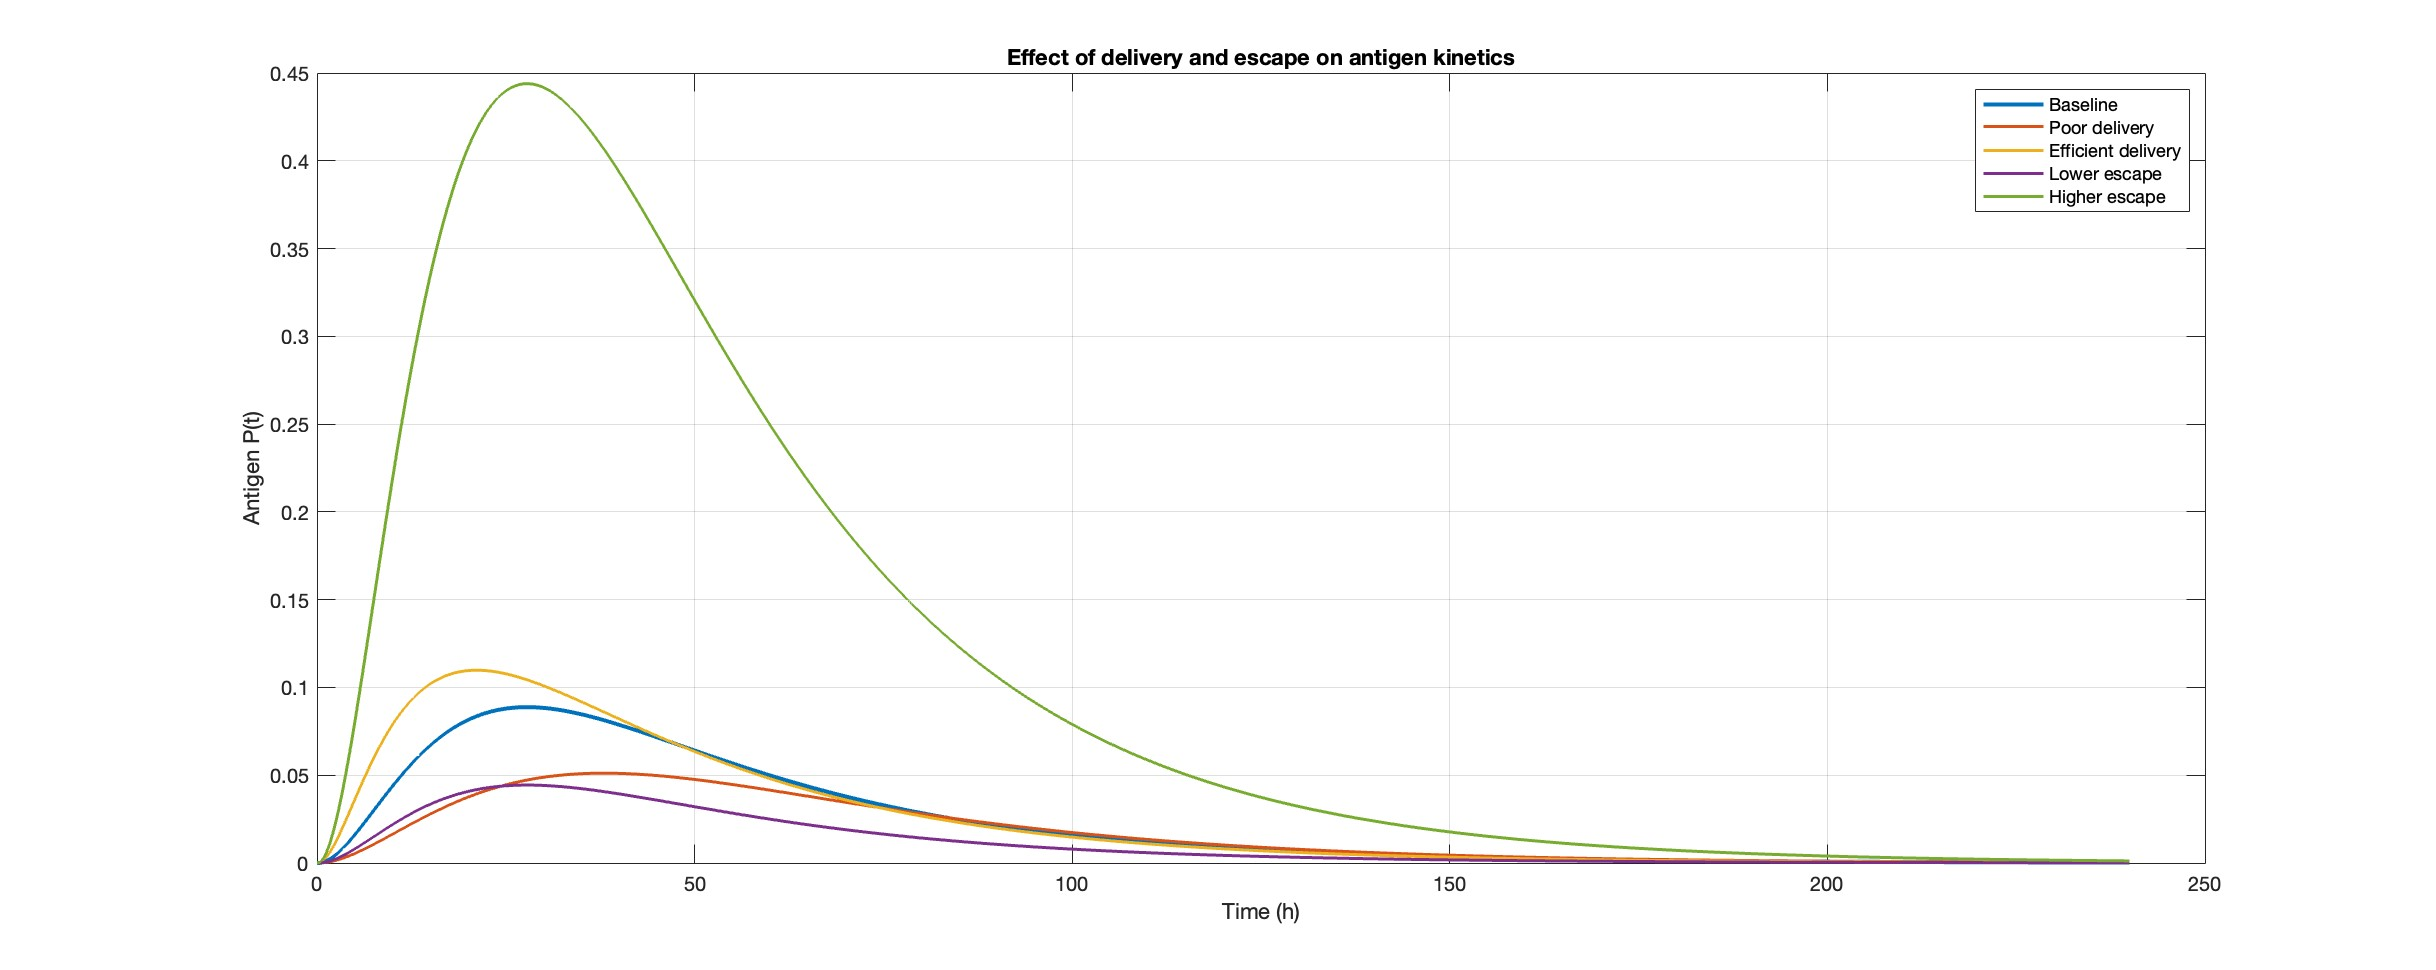
\includegraphics[width = \textwidth]{figures/Del&Esc.jpg}
    \caption{Effects of delivery and escape on antigen expression}
    \label{fig:delesc}
\end{figure}

\begin{figure}[H]
    \centering
    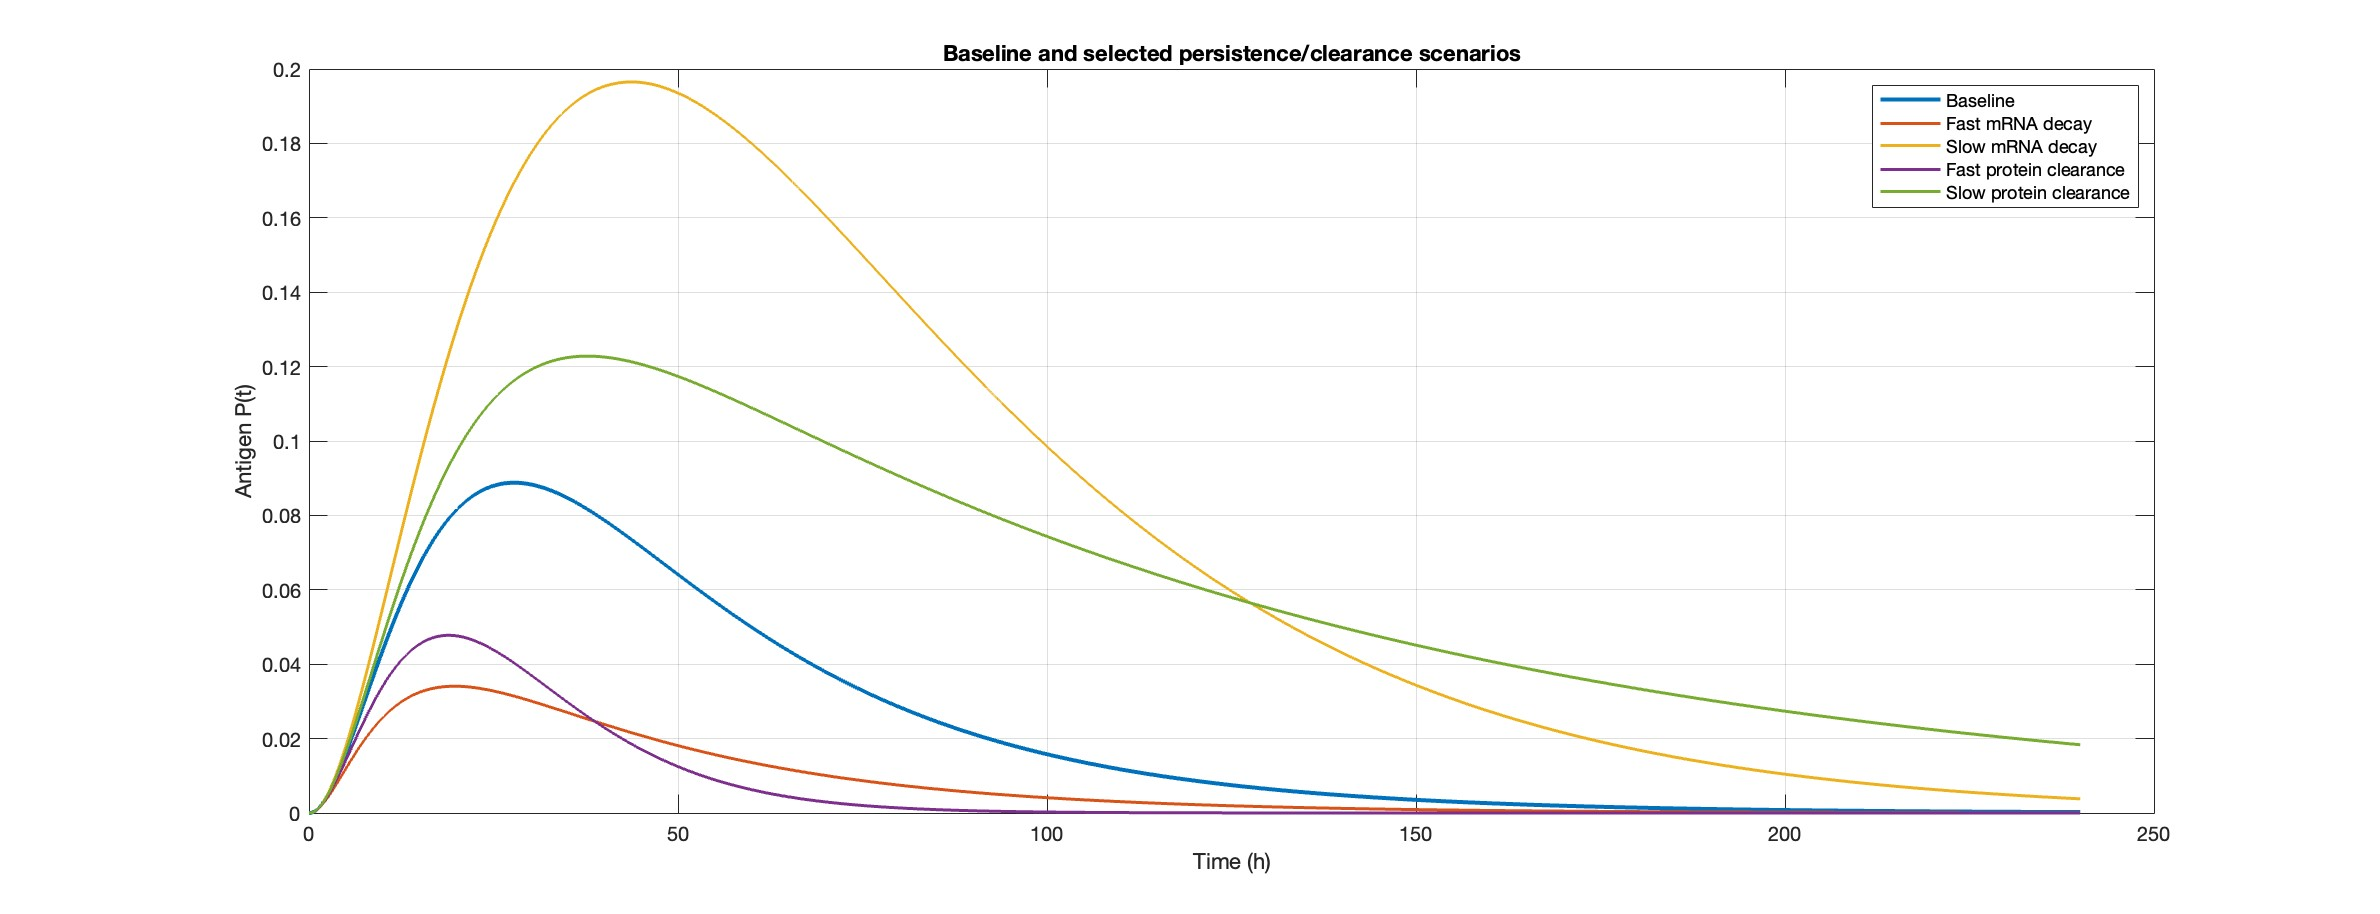
\includegraphics[width = \textwidth]{figures/P(t)_scenarios.jpg}
    \caption{Baseline and selected scenarios}
    \label{fig:Ptscenarios}
\end{figure}

How these shifts map to the requested interpretation:
\begin{itemize}
    \item \textbf{Peak height} increases strongly with $k_{\mathrm{tl}}$, $f_{\mathrm{esc}}$, and (in many regimes) faster early supply via $k_{\mathrm{up}}$.
    \item \textbf{Time to peak} shifts earlier with faster uptake and faster clearance; shifts later with slower mRNA decay and slower protein clearance.
    \item \textbf{Duration} (FWHM / long tail) lengthens with slower mRNA decay and slower protein clearance; it also lengthens when uptake is slow but persistent (depot-limited regime).
    \item $\mathrm{AUC}_P$ follows the derived multiplicative scaling $D_0f_{\mathrm{up}}f_{\mathrm{esc}}\bigl(k_{\mathrm{tl}}/(k_{\mathrm{deg}}k_{\mathrm{clr}})\bigr)$, so changing $f_{\mathrm{esc}}$ by an order of magnitude changes AUC by an order of magnitude.
\end{itemize}

\subsection*{Burst vs sustained delivery strategies}

Two stylized strategies implemented by changing depot/uptake parameters:
\begin{itemize}
    \item \textbf{Burst-like}: rapid uptake and rapid depot loss (e.g., large $k_{\mathrm{up}}$, $k_{\mathrm{clr},L}$).
    \item \textbf{Sustained-like}: slower uptake with lower depot clearance (smaller $k_{\mathrm{up}}$, $k_{\mathrm{clr},L}$).
\end{itemize}

Illustrative outputs:
\begin{itemize}
    \item Burst: earlier peak ($\sim 20$ h), modestly narrower curve.
    \item Sustained: later peak ($\sim 43$ h), broader curve with longer tail.
\end{itemize}

Such differences are consistent with observations that expression kinetics depend on local stability/availability and trafficking, not only total dose. \parencite{pardi2015expressionKinetics}

\subsection*{Matlab simulation psuedocode}
\inputminted[linenos, frame=single, breaklines, baselinestretch=1.2, fontsize=\small]{matlab}{sections/code.txt}